\subsection{Portes, \glsfmtlong{gru} et \glsfmtlong{lstm}}

Pour une grande partie des problèmes d'apprentissage \gls{s2s}, les séquences peuvent être très longues.
Le mémoire à court terme constitue donc un véritable obstacle pour l'utilisation des \glspl{rnn} simples en pratique.
Une approche de le contourner qui a eu un énorme succès expérimental, 
est l'introduction d'un mécanisme de contrôle sur la boucle de rétroaction (Voire Figure~\ref{fig.rnn-gate}).
Ce mécanisme est généralement implémenté avec des \emph{portes},
des unités entraînables qui peuvent réguler le flux d'information dans la couche récurrente.
On parle alors d'\emph{\gls{rnn} à portes}.
Dans cette section, nous explorons les deux variants les plus utilisés d'\glspl{rnn} à portes :
le \gls{gru} et le \gls{lstm}. 


\begin{figure}[htb]
    \begin{center}
        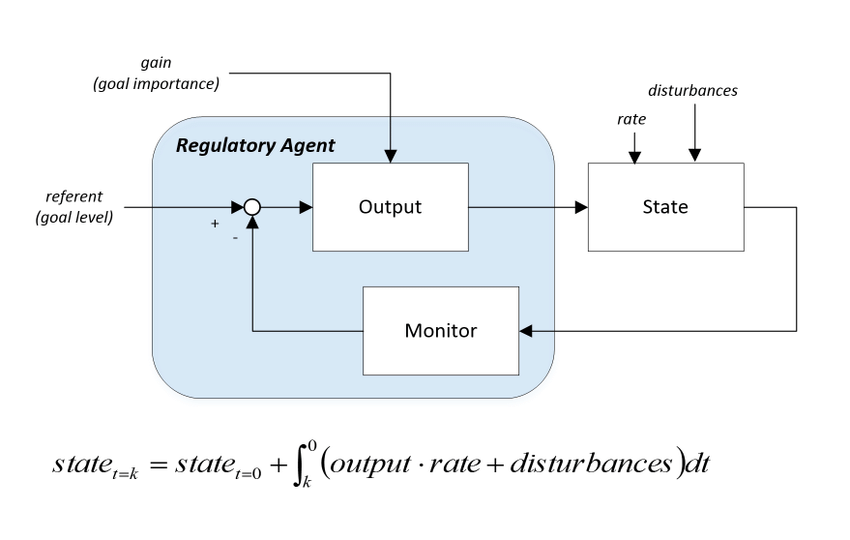
\includegraphics[width=8cm]{assets/images/gated-feedback.png}
    \end{center}
    \caption{Forme générale d'un \glsfmtshort{rnn} à portes.}
    \label{fig.rnn-gate}
\end{figure}

\subsubsection{\Glsfmtlong{gru}}

Le \gls{gru}, introduit par~\cite{Cho_van_Merrienboer_Bahdanau_Bengio_2014}, 
est une architecture récurrente à portes très simple (Voir Figure~\ref{fig.gru-circuit}).
Elle utilise deux portes.
La première est la porte de réinitialisation ((\(r\) dans la figure~\ref{fig.gru-circuit})).
Elle détermine le point auquel l'information sur le passé peut se propager
(quand \(r=0\), pas de propagation et quand \(r=1\), propagation totale).
Sa sortie s'appelle \emph{l'état candidat} (\(\tilde{h}\) dans la figure).
La deuxième est la porte de mise à jour (\(z\) dans la figure).
Elle détermine les contributions respectives de l'état candidat et l'état passé
(si \(z=0\), seul l'état candidat contribue et si \(z=1\), seule l'état courant contribue).
Sa sortie est la sortie globale du \gls{gru}~\cite{Cho_van_Merrienboer_Bahdanau_Bengio_2014}.


\begin{figure}[htb]
    \begin{center}
        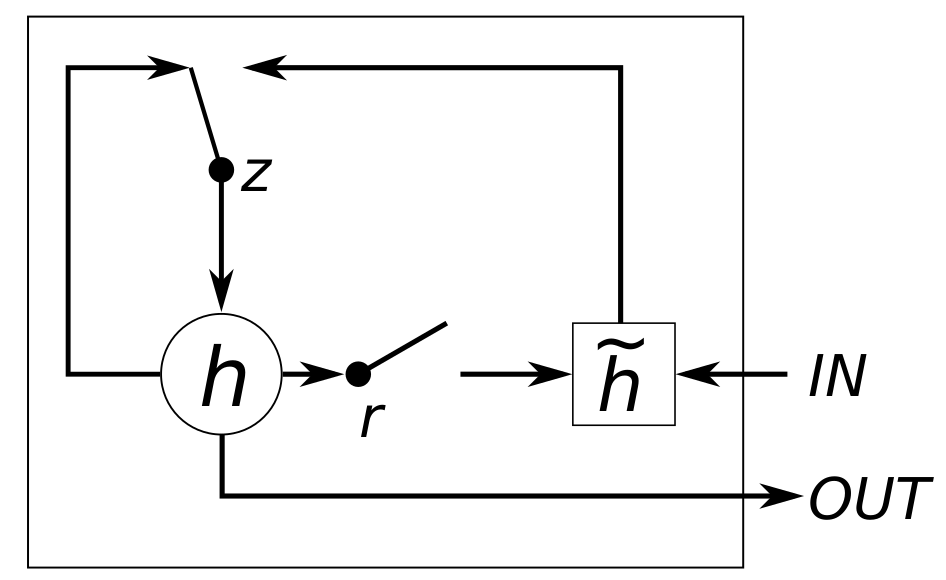
\includegraphics[width=8cm]{assets/images/gru-circuit.png}
    \end{center}
    \caption{Architecture interne d'un \glsfmtshort{gru}~\cite[Fig. 1b]{Chung_Gulcehre_Cho_Bengio_2014}}
    \label{fig.gru-circuit}
\end{figure}

Le fonctionnement des portes d'un \gls{gru} est simple.
Leurs valeurs sont calculées à partir de l'entrée et de l'état courants par
les équations~\ref{eq.gru-update} et \ref{eq.gru-reset}, 
où \(\sigma\) est la fonction \emph{sigmoïde}%
\footnote{\(\sigma:\reals\to\reals, x\mapsto\frac{1}{1+e^{-x}}\)}
et \(\odot\) et le produit d'Hadamard%
\footnote{Pour \(u, v\in\reals^n\), \(u\odot v\in\reals^n\) et \((u\odot v)_i = u_i v_i\)}.
\begin{eqnarray}
    \label{eq.gru-update}
    z^{(t)}  &=&\sigma\left(W_z x^{(t)}+U_z h^{(t-1)}+b_z\right) \\
    \label{eq.gru-reset}
    r^{(t)}  &=&\sigma\left(W_r x^{(t)}+U_r h^{(t-1)}+b_r\right) \\
    \label{eq.gru-candidate}
    \tilde{h}^{(t)}  &=&\phi\left(W_h x^{(t)}+U_h\left(r^{(t)} \odot h^{(t-1)}\right)+b_h\right) \\
    \label{eq.gru-out}
    h^{(t)}  &=&z^{(t)} \odot h^{(t-1)}+\left(1-z^{(t)}\right) \odot \tilde{h}^{(t)}
\end{eqnarray}
L'état candidat est calculé à partir de l'entrée et l'état pondéré par la porte de réinitialisation
par l'équation~\ref{eq.gru-candidate}, où \(\phi\) est la fonction d'activation.
Finalement, l'état futur (la sortie) est la moyenne pondérée par \(z\) 
de l'état courant et l'état candidat~\cite{Cho_van_Merrienboer_Bahdanau_Bengio_2014}.
Notons que le \gls{gru} devient un \gls{rnn} simple 
si les portes de réinitialisation et de mise à jour sont respectivement fixés à \(1\) et \(0\)%
~\cite{Fathi_2021}.

\subsubsection{\Glsfmtlong{lstm}}

Il s'agit de l'une des premières architectures récurrentes à protes%
~\cite{Chung_Gulcehre_Cho_Bengio_2014}.
Elle a été introduite par~\cite{Hochreiter_Schmidhuber_1997}.
Un \gls{lstm} implémente trois portes : 
une porte d'entrés (\(i\)), une porte d'oublie (\(f\)) et une porte de sortie (\(o\))%
(Voir Figure~\ref{fig.lstm-circuit}).

\begin{figure}[htb]
    \begin{center}
        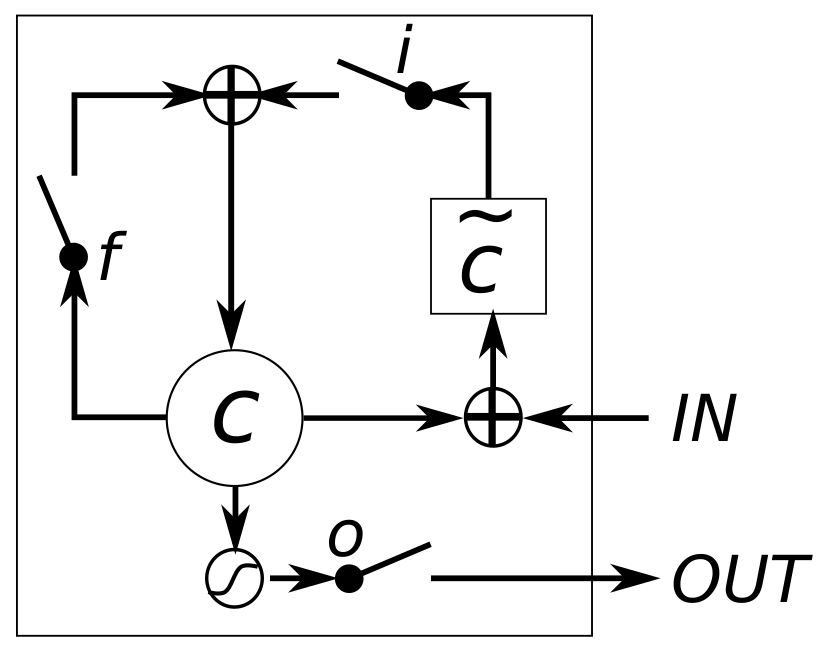
\includegraphics[width=8cm]{assets/images/lstm-circuit.png}
    \end{center}
    \caption{Architecture interne d'un \glsfmtshort{lstm}~\cite[Fig. 1a]{Chung_Gulcehre_Cho_Bengio_2014}}
    \label{fig.lstm-circuit}
\end{figure}

Le fonctionnement des portes est similaire à celui du \gls{gru}.
Les équations~\ref{eq.lstm-forget}--\ref{eq.lstm-h} le montrent en détails%
\footnote{\(\tanh:\reals\to\reals, x\mapsto \frac{e^x - e^{-x}}{e^x + e^{-x}}\)}
~\cite{Hochreiter_Schmidhuber_1997}.

\begin{eqnarray}
    \label{eq.lstm-forget}
    f^{(t)} &=&\sigma\left(W_f x^{(t)}+U_f h^{(t-1)}+b_f\right) \\
    \label{eq.lstm-input}
    i^{(t)} &=&\sigma\left(W_i x^{(t)}+U_i h^{(t-1)}+b_i\right) \\
    \label{eq.lstm-out}
    o^{(t)} &=&\sigma\left(W_o x^{(t)}+U_o h^{(t-1)}+b_o\right) \\
    \label{eq.lstm-ctilde}
    \tilde{c}^{(t)} &=&\tanh\left(W_c x^{(t)}+U_c h^{(t-1)}+b_c\right) \\
    \label{eq.lstm-c}
    c^{(t)} &=&f^{(t)} \odot c^{(t-1)}+i^{(t)} \odot \tilde{c}^{(t)} \\
    \label{eq.lstm-h}
    h^{(t)} &=&o^{(t)} \odot \phi\left(c^{(t)}\right)
\end{eqnarray}

\subsubsection{Évaluation des \glsfmtlongpl{rnn}}

Nous avons établi que les \glspl{rnn} simples souffrent du mémoire à court terme%
~\cite{Bengio_Simard_Frasconi_1994,Pascanu_Mikolov_Bengio}.
En utilisant les portes pour contrôler le flux d'information,
les \glspl{gru} et \glspl{lstm} résolvent le problème au coût d'une architecture plus complexe.
Ils ont des performances similaires est largement meilleures que celle des \glspl{rnn}%
~\cite{Chung_Gulcehre_Cho_Bengio_2014}.

Cependant, toutes les architectures récurrentes présentent un problème fondamental : 
elles fonctionnent séquentiellement.
Bien que cela les rend naturellement mieux adaptées à la modélisation de séquences,
il les rend aussi quasi impossibles à paralléliser pour exploiter des architectures parallèles (GPU).
Par conséquent, l'entraînement des \glspl{rnn} est extrêmement lent~\cite{Stahlberg_2020}.
